\begin{figure}[htbp]
\centering
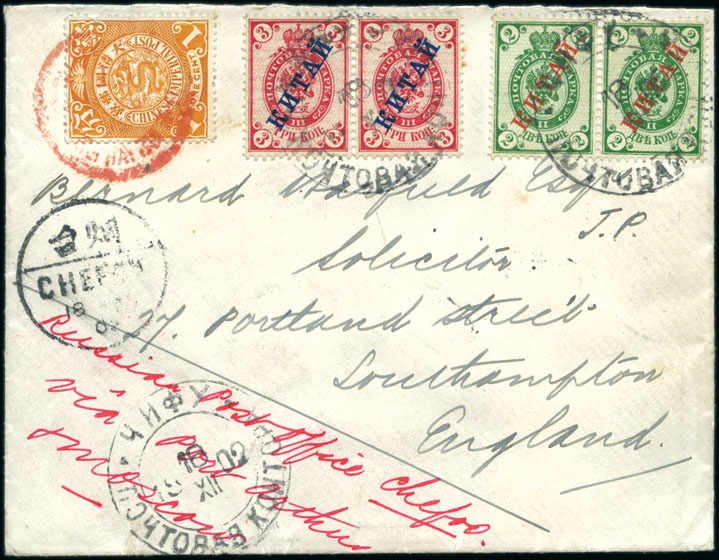
\includegraphics[width=.95\textwidth]{../russian-post-offices-in-china/10100.jpg}
\caption{
10100	CHEFOO: 1902 Cover to England from a crew member on board 
British warship HMS "Amphitrite" (printed on the reverse) at the Crown 
Colony of Wei Hai Wei, endorsed "Russian Post Office Chefoo / via 
Port Arthur / Moscow", with China 1c Dragon tied by bilingual 
"LIU-KUNG-TAO / WEI-HAI-WEI" cds in red, paying the rate to Chefoo 
where it was transferred to the Russian P.O. and franked with pairs of 
"KITAI" 2k and 3k tied by Chefoo 18.12.02 cds (T\&S type 1, Gregorian calendar), 
with different strike on reverse (T\&S type 2, Julian calendar), 
Southampton bs, a rare and attractive mixed country franking
\euro 800.00 
}  
\end{figure} 

\begin{figure}[htbp]
\centering
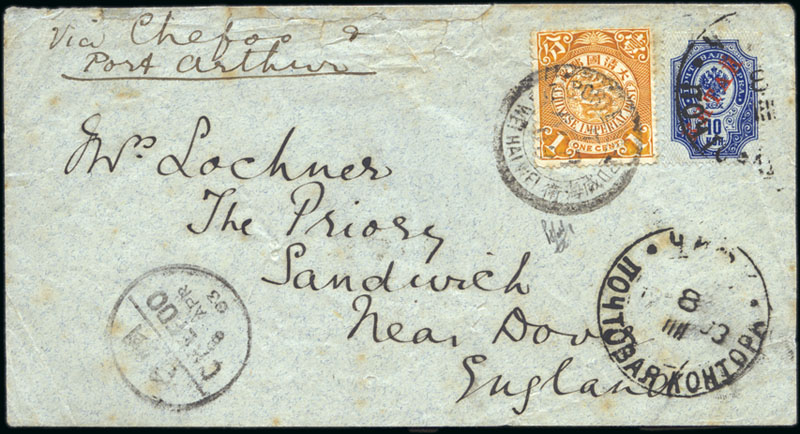
\includegraphics[width=.95\textwidth]{../russian-post-offices-in-china/10101.jpg}
\caption{
10101	CHEFOO: 1903 Cover to England endorsed "via Chefoo \& Port Arthur", 
with China 1c Dragon tied by bilingual / WEI HAI WEI" cds, sent via Chefoo 
where it was transferred to the Russian P.O. and franked with "KITAI" 10k 
tied by Chefoo 8.4.03 cds (T\&S type 1), Sandwich bs

Note: This Port Edward cds was in use only from April 1903 to January 1904. 
This item is dated a day earlier than the earliest date recorded by 
M. Goldsmith \& C. Goodwyn in "The Crown Colony of Wei Hei Wei"
\euro 500.00 
}  
\end{figure} 

\begin{figure}[htbp]
\centering
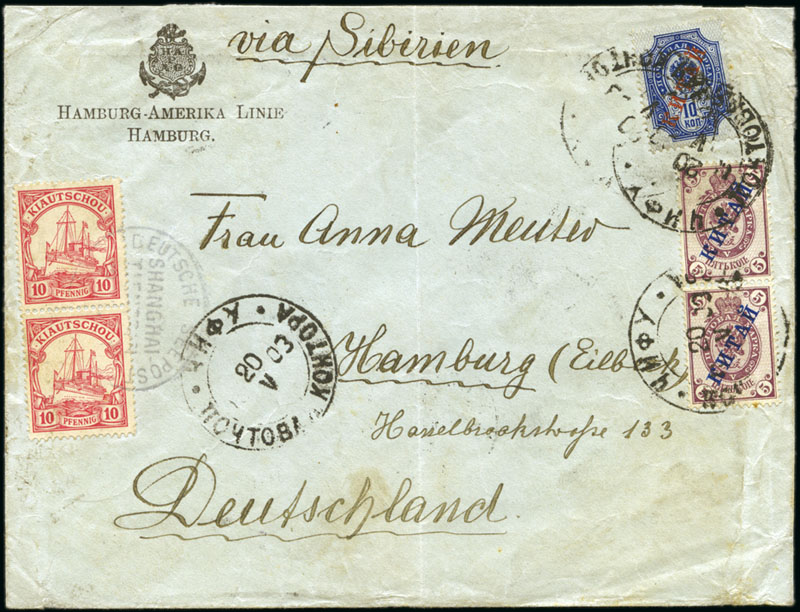
\includegraphics[width=.95\textwidth]{../russian-post-offices-in-china/10102.jpg}
\caption{
10102 CHEFOO: 1903 Hamburg-America Line printed envelope franked with 
Kiautschou 10pf vertical pair tied by "DEUTSCHE SEEPOST / SHANGHAI / TIENTSIN" 
oval ds, transferred to the Russian P.O. at Chefoo and franked with "KITAI" 5k (2) 
and 10k tied by Chefoo 20.5.03 cds (T\&S type 1), with Moscow and 
Hamburg bs, a possibly unique and spectacular combination.
Note: From Chefoo a daily steamer service connected the newly 
built Chinese Eastern Railway at Port Arthur and thence the Trans-Siberian 
railway to Europe.
\euro 4,000.00
}  
\end{figure} 

\begin{figure}[htbp]
\centering
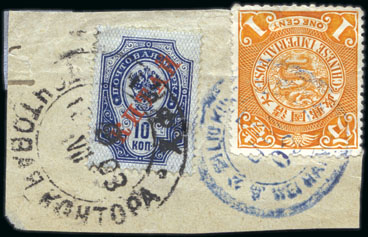
\includegraphics[width=.50\textwidth]{../russian-post-offices-in-china/10103.jpg}
\caption{
10103 CHEFOO: Fragment with China 1c tied by "LIU KUNG TAO / WEI HAI WEI" cds 
in blue, and "KITAI" 10k tied by Chefoo 9.7.03 cds (T\&S type 1), fine
\euro 40.00 
}  
\end{figure} 

\begin{figure}[htbp]
\centering
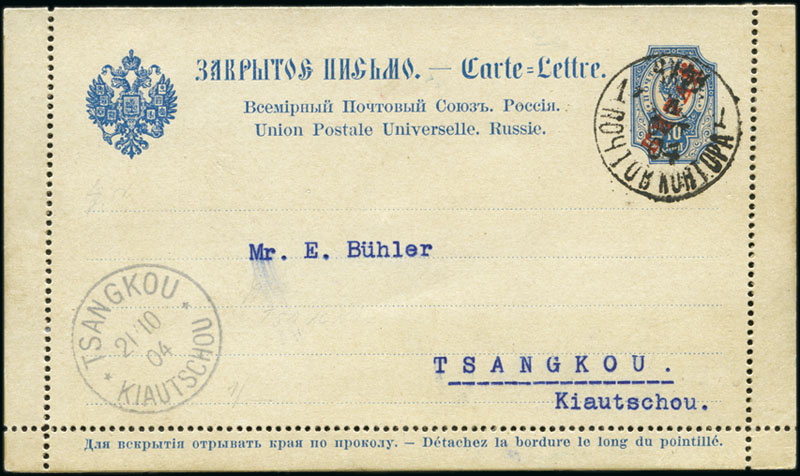
\includegraphics[width=.95\textwidth]{../russian-post-offices-in-china/10104.jpg}
\caption{
10104	CHEFOO: 1904 "KITAI" 10k letter card to the German Colony Tsangkow, 
Kiaochow, cancelled by Chefoo 4.10.04 cds (T\&S type 2), with 
Tsangkou / Kiautschou arrival cds adjacent, very fine and unusual destination
\euro 150.00
}  
\end{figure} 



\begin{figure}[htbp]
\centering
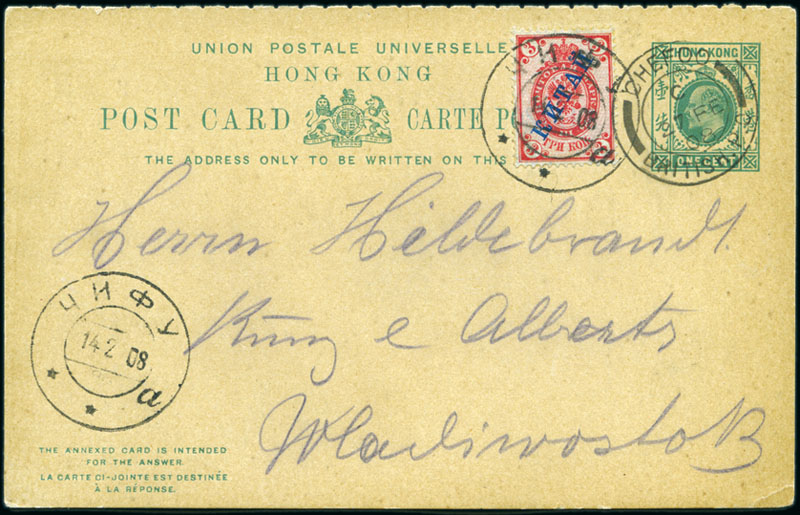
\includegraphics[width=.95\textwidth]{../russian-post-offices-in-china/10105.jpg}
\caption{
10105	CHEFOO: 1908 Hong Kong 1c reply paid card to Vladivostok, 
franked with "KITAI" 3k, with imprint cancelled by British P.O. 
Chefoo 27.2.08 cds and stamp tied by Russian P.O. Chefoo cds on the same 
day, very unusual.
\euro 200.00
}  
\end{figure} 

  
\begin{figure}[htbp]
\centering
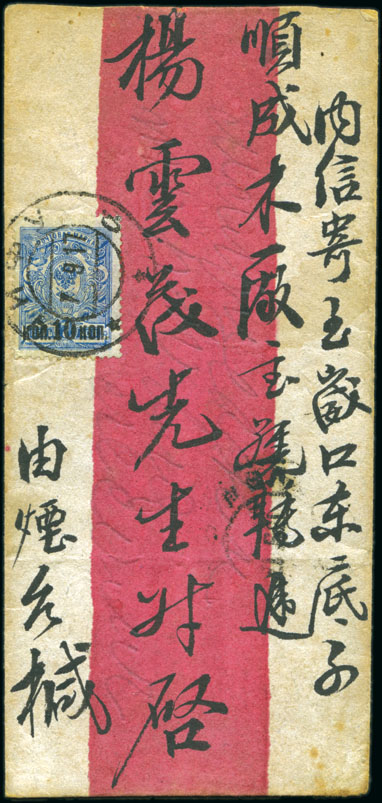
\includegraphics[width=.45\textwidth]{../russian-post-offices-in-china/10106.jpg}
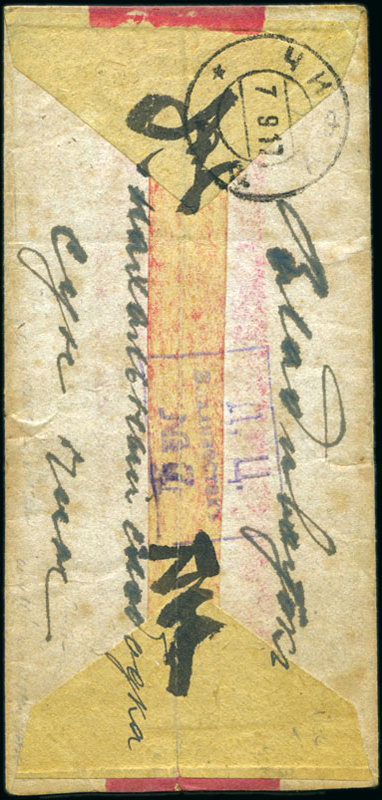
\includegraphics[width=.45\textwidth]{../russian-post-offices-in-china/10106-1.jpg}
\caption{
10106 CHEFOO: 1917 Native cover to Vladivostok with 1916 10k on 7k provisional 
tied by Chefoo 7.9.17 cds (Tchilinghirian type 2A), with Vladivostok cds and 
violet censor cachet on reverse, a rare franking, there is no previous record 
of the use of the 1916 provisionals in China proper (only in Mongolia and Sinkiang).
\euro 400.00
}  
\end{figure}   
  
\begin{figure}[htbp]
\centering
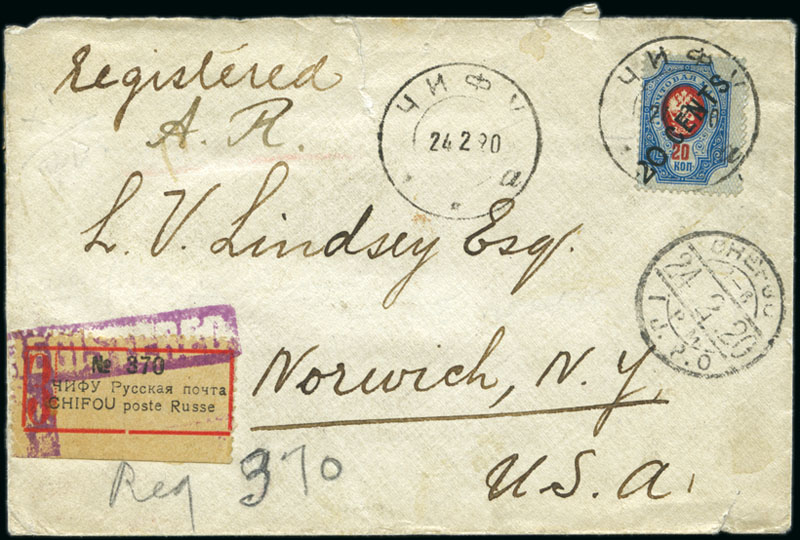
\includegraphics[width=.95\textwidth]{../russian-post-offices-in-china/10107.jpg}
\caption{
10107	CHEFOO: 1920 Registered cover sent to Norwich, New York, USA with 20 
CENTS on 20k surcharged issue, tied by Chefoo 24.2.20 cds (T\&S type 3A), 
with reg'd label in Russian and French adjacent \& tied by American 
type negative registered cachet, plus manuscript "Registered A.R." \& IJPO cds 
of Chefoo, a rare use of the surcharged issue
\euro 200.00
}  
\end{figure}    
  
  
  
  
  
  
  
  
  
  
  
                    